% Sibling types: full, half, step and adoptive siblings (all relative to A).
\documentclass[tikz, border=4mm]{standalone}
% Shared style for the pedigree components (\input by components/pedigree_*.tex).
\usepackage[T1]{fontenc}
\usepackage{lmodern}
\usepackage[default]{sourcesans}
\usetikzlibrary{positioning, calc}

% one palette for every relationship type (Okabe-Ito, colour-blind safe)
\definecolor{cFull}{HTML}{0072B2}   % full siblings
\definecolor{cHalf}{HTML}{009E73}   % half-siblings
\definecolor{cStep}{HTML}{D55E00}   % step-siblings
\definecolor{cAdopt}{HTML}{56B4E9}  % adoptive siblings
\definecolor{cCous}{HTML}{CC79A7}   % 1st cousins
\definecolor{cCoc}{HTML}{E69F00}    % co-cousins
\definecolor{ink}{HTML}{1F2328}
\definecolor{leaf}{HTML}{DDE3EA}

\tikzset{
  ped/.style={draw=ink, line width=1.2pt},
  male/.style={ped, rectangle, minimum size=7.5mm, inner sep=0pt, fill=#1, font=\small\bfseries},
  female/.style={ped, circle, minimum size=8.2mm, inner sep=0pt, fill=#1, font=\small\bfseries},
  male/.default=white, female/.default=white,
  line/.style={ped},
  adopted/.style={ped, dash pattern=on 4pt off 3pt},
  rel/.style={line width=3.2pt, rounded corners=6pt, line cap=round},
  rellab/.style={font=\small\bfseries, fill=white, inner sep=1.5pt},
}
% connector from x1 to x2 at depth d below the leaf row (y = base), label in the middle
% \connect{colour}{x1}{x2}{depth}{label}{label position: on | below}
\newcommand{\connect}[6]{%
  \draw[rel, #1] (#2,\base) -- (#2,\base-#4) -- (#3,\base-#4) -- (#3,\base);
  \ifx#6b\node[rellab, text=#1, below=1mm] at ($(#2,\base-#4)!0.5!(#3,\base-#4)$) {#5};%
  \else\node[rellab, text=#1] at ($(#2,\base-#4)!0.5!(#3,\base-#4)$) {#5};\fi}

\begin{document}
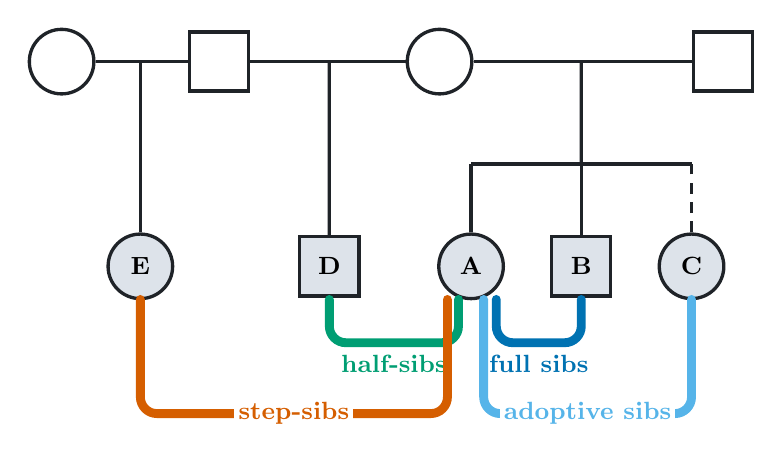
\begin{tikzpicture}[x=1cm, y=1cm]
\def\gP{0}\def\gL{-2.6}\def\base{\gL-0.42}
% parents: a woman with two partners; her second partner already had a child
\node[female] (m2) at (0,\gP) {};
\node[male]   (f2) at (2,\gP) {};
\node[female] (m1) at (4.8,\gP) {};
\node[male]   (f1) at (8.4,\gP) {};
\draw[line] (m2) -- (f2);  \draw[line] (f2) -- (m1);  \draw[line] (m1) -- (f1);
% children (leaves)
\node[female=leaf] (e) at (1,\gL)   {E};
\node[male=leaf]   (d) at (3.4,\gL) {D};
\node[female=leaf] (a) at (5.2,\gL) {A};
\node[male=leaf]   (b) at (6.6,\gL) {B};
\node[female=leaf] (c) at (8.0,\gL) {C};
\draw[line] ($(m2)!0.5!(f2)$) -- (e.north);
\draw[line] ($(f2)!0.5!(m1)$) -- (d.north);
\draw[line] ($(m1)!0.5!(f1)$) -- (6.6,\gL+1.3);
\draw[line] (5.2,\gL+1.3) -- (8.0,\gL+1.3);
\draw[line] (a.north) -- (5.2,\gL+1.3);
\draw[line] (b.north) -- (6.6,\gL+1.3);
\draw[adopted] (c.north) -- (8.0,\gL+1.3);      % adopted: dashed line of descent
% relationships of A
\connect{cFull}{5.52}{6.6}{0.55}{full sibs}{b}
\connect{cAdopt}{5.36}{8.0}{1.45}{adoptive sibs}{o}
\connect{cHalf}{5.04}{3.4}{0.55}{half-sibs}{b}
\connect{cStep}{4.9}{1}{1.45}{step-sibs}{o}
\end{tikzpicture}
\end{document}
